\documentclass[9pt, xcolor={usenames, dvipsnames}]{beamer}

\usepackage[sfdefault]{roboto}
\usepackage[utf8]{inputenc}
\usepackage[T1]{fontenc}
\usepackage{palatino}

\usepackage{styles/fluxmacros}
\usefolder{styles}
% Use Flux theme v0.1 beta
% Available style: asphalt, blue, red, green, gray 
\usetheme[style=flux]{flux}
\usetikzlibrary{hobby}

\usepackage{booktabs}
\usepackage{colortbl}
\usepackage{empheq}
\usepackage{xcolor}

\usepackage{caption}
\usepackage{subcaption}
\setbeamertemplate{caption}[numbered]
\captionsetup[figure]{font=footnotesize,labelfont=footnotesize}

\title{Enclosure methods for safe localisation}
% \subtitle{Application to boat control using bathymetry}
\author{Quentin Brateau}
\institute{ENSTA Bretagne~~~·~~~Agence Innovation Défense\\[0.5cm]
\includegraphics[width=0.5\textwidth]{images/logos_title_page.png}}
\date{\today}
\titlegraphic{images/logos_bw.png}

% \usepackage[usenames, dvipsnames]{xcolor}
\usepackage{pifont}
\newcommand{\cmark}{\textcolor{ForestGreen}{\ding{51}}}
\newcommand{\xmark}{\textcolor{Red}{\ding{55}}}

\usepackage{graphicx}
\usepackage{multimedia}
\usepackage{tikz}
\usetikzlibrary{overlay-beamer-styles}

\tikzset{
	block/.style = {draw, fill=white, rectangle, minimum height=2em, minimum width=5em},
	tmp/.style  = {coordinate}, 
	sum/.style= {draw, fill=white, circle, node distance=1cm},
	input/.style = {coordinate},
	output/.style= {coordinate},
	pinstyle/.style = {pin edge={to-,thin,black}},
	highlight/.style={alt=<#1>{fill=red!30}}
}

\begin{document}

	\titlepage

	\begin{frame}
		\frametitle{Table of contents}
		\tableofcontents
	\end{frame}

	\section{Introduction}
	\AllSectionsWithTitlePage

		\subsection{Context}
			\begin{frame}{Context}{Safe and Resilient control}
				\centering
				\begin{minipage}[c]{0.6\textwidth}
					\onslide<1->{
						\begin{block}{Safe navigation}
							\begin{itemize}
								\item Guaranteed state estimation
								\item Ensure non-collision
							\end{itemize}
						\end{block}
					}
					\onslide<2->{
						\begin{block}{Resilient navigation}
							\begin{itemize}
								\item Keeps working with the loss of sensors
								\item Detect sensor inconsistencies
							\end{itemize}
						\end{block}
					}
				\end{minipage}
				\hfill
				\begin{minipage}[c]{0.35\textwidth}
					\begin{figure}
						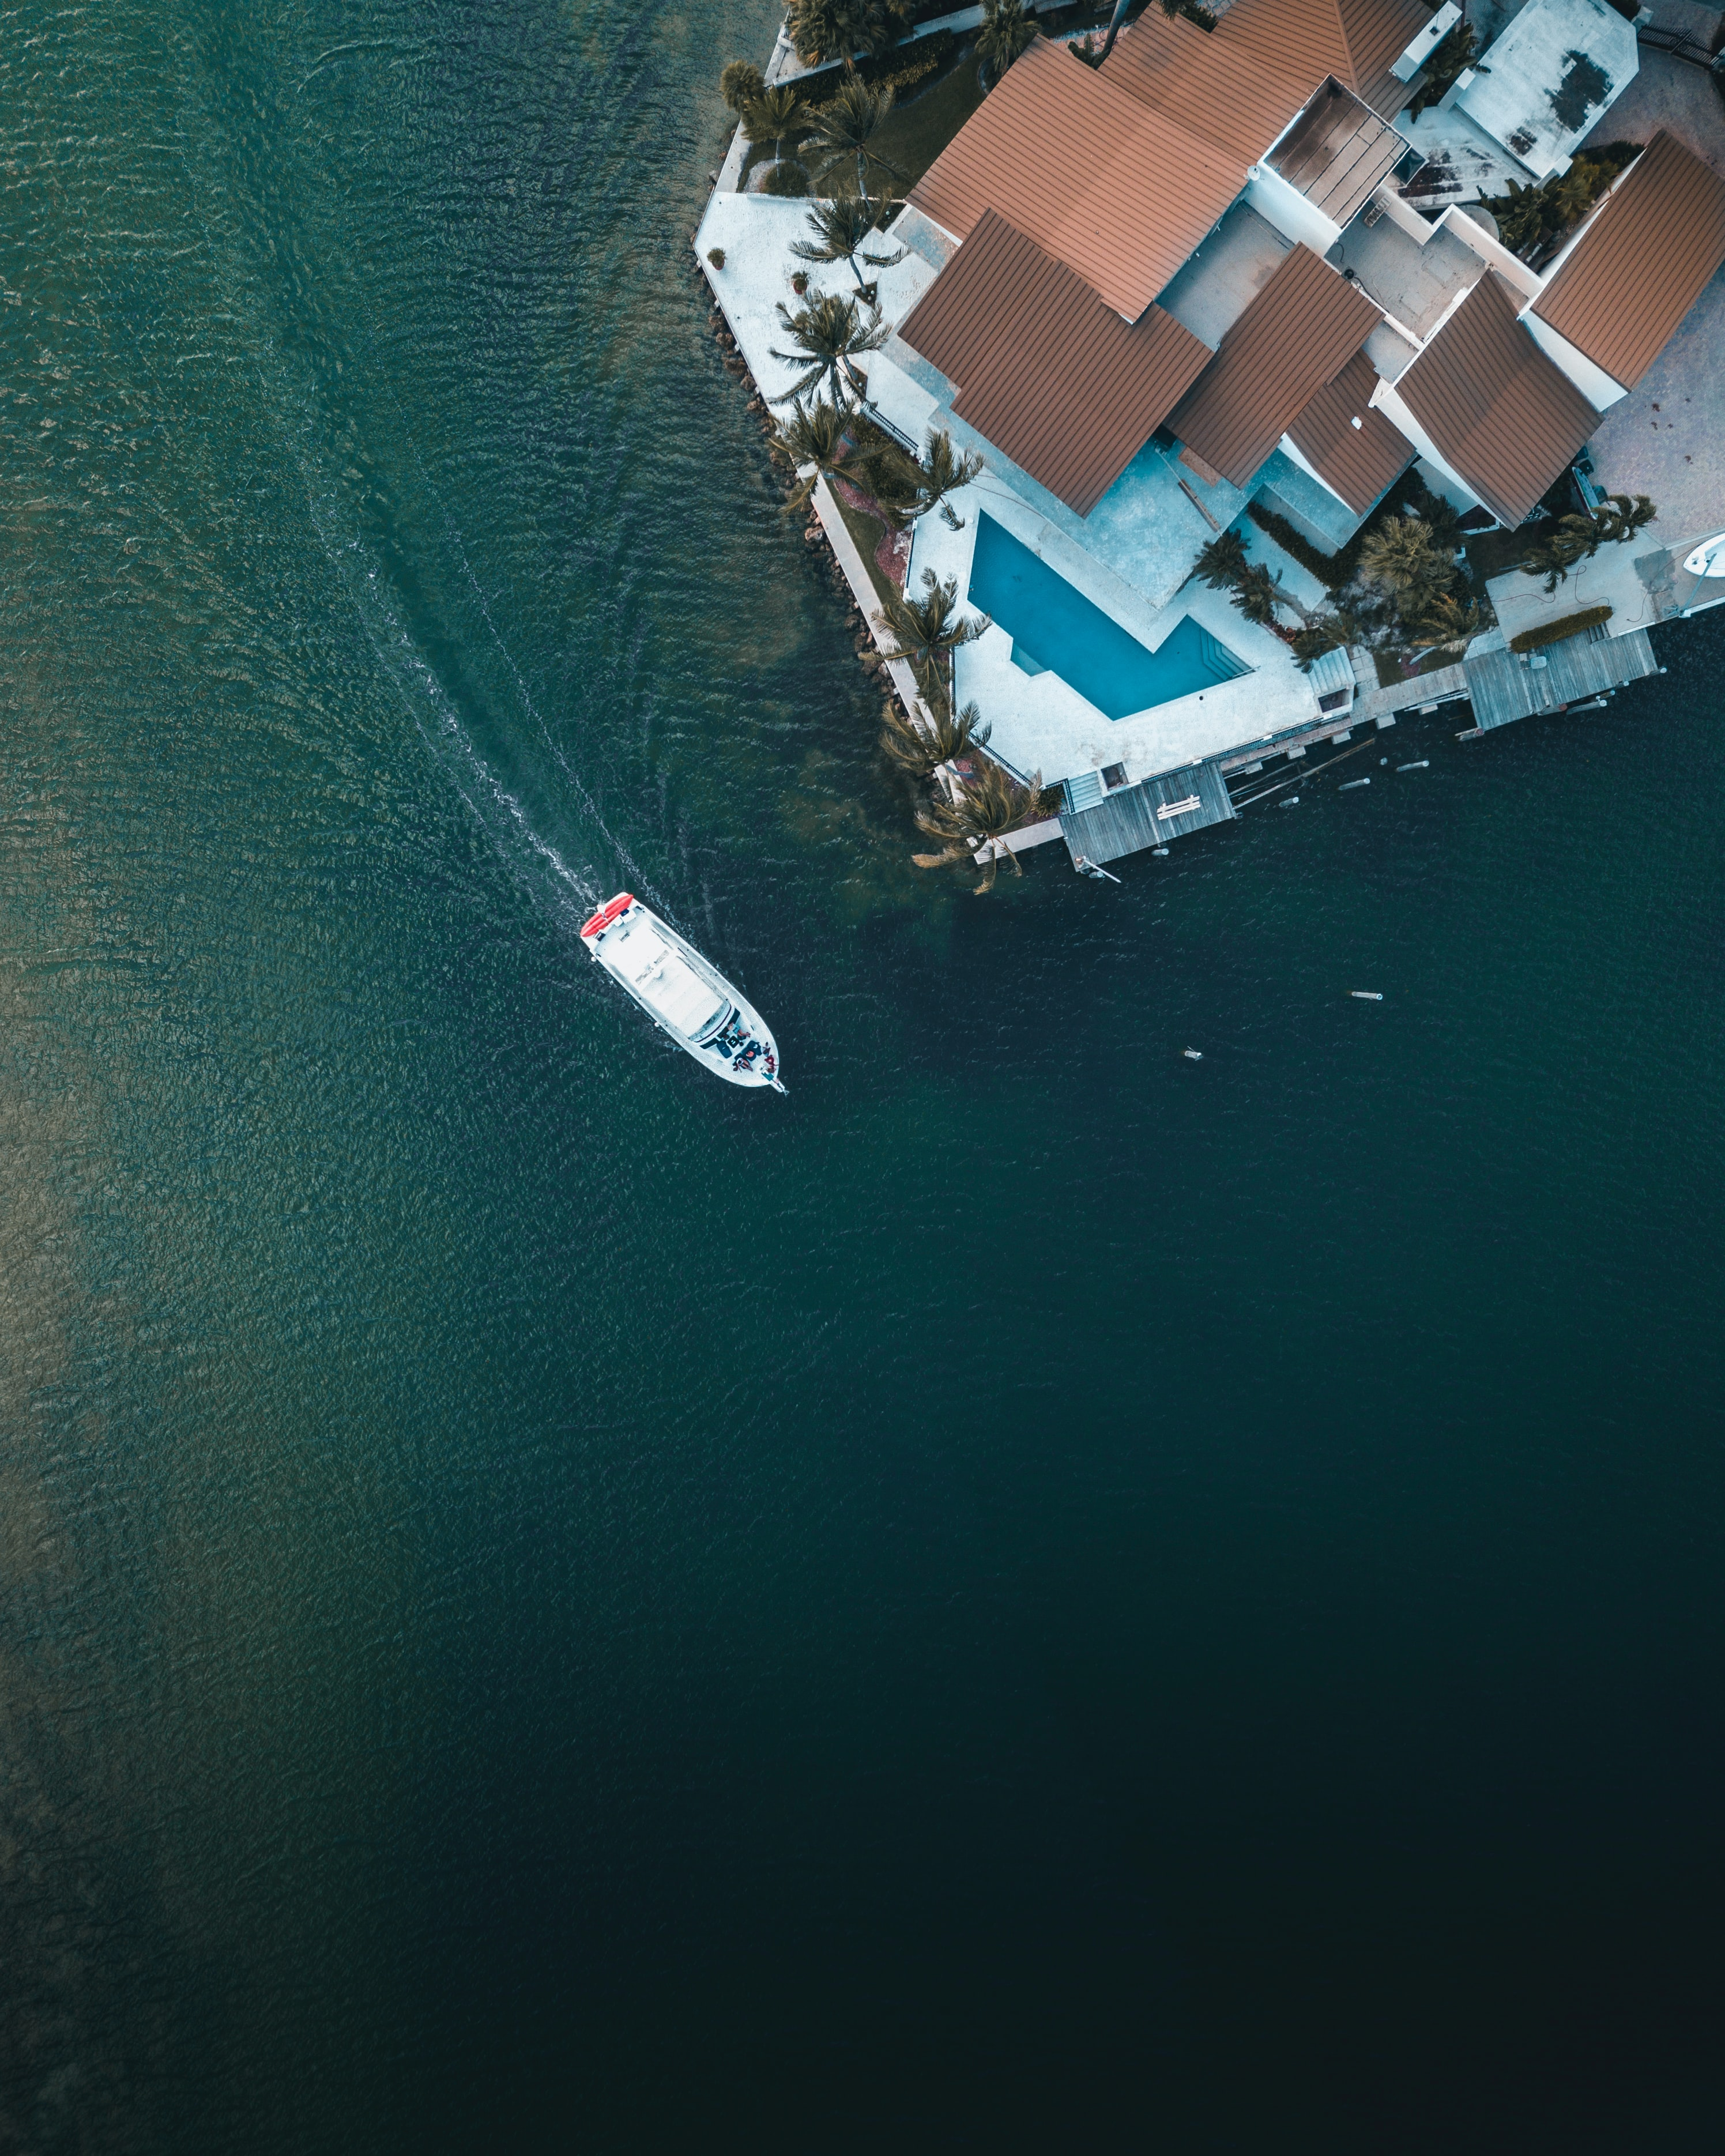
\includegraphics[width=\textwidth, trim=100 0 200 0, clip]{images/boat_view.jpg}
						\caption{Sailing boat}
					\end{figure}
				\end{minipage}
			\end{frame}

	\section{Formalism}

		\subsection{State Equation}

			\begin{frame}{Formalism}{State Equation}
				\centering
				\begin{minipage}{0.6\textwidth}
					\onslide<1->{
						\begin{block}{State Equation}
							System defined by state equation
							\begin{empheq}[left=\empheqlbrace]{align}
								\dot{x} & = f(x, u) &(evolution) \\
								y & = g(x, u) &(observation)
							\end{empheq}
						\end{block}
					}
					\onslide<2->{
						\begin{block}{Application}
							\begin{itemize}
								\item Dynamic knowledge of the system
								\item Control the system
								\item Simulate the system
							\end{itemize}
						\end{block}
					}
				\end{minipage}
			\end{frame}

		\subsection{Guidance-Navigation-Control systems}

			\begin{frame}{Introduction}{Guidance-Navigation-Control systems}
				\centering
				\begin{figure}[t]
					\centering
					\resizebox*{0.6\textwidth}{!}{
						\begin{tikzpicture}[auto, node distance=2.5cm, >=latex']
							\node [input, name=rinput] (rinput) {};
							\node [block, right=1cm of rinput, highlight=4] (guidance) {Guidance};
							\node [block, right of=guidance, highlight=3] (control) {Control};
							\node [block, right of=control, highlight=1] (system) {System};
							\node [block, below left=1cm and -0.5cm of system, highlight=2] (navigation) {Navigation};
							\node [output, right=1cm of system] (output) {};
							\draw [->] (rinput) -- node [name=p] {$p$}(guidance);
							\draw [->] (guidance) -- node [name=r] {$r$}(control);
							\draw [->] (control) -- node [name=u] {$u$}(system);
							\draw [->] (system) -- node [name=y] {$y$}(output);
							\draw [->] (y) |- (navigation);
							\draw [->] (navigation) -| node[name=xhat1, pos=0.9] {$\hat{x}$} (control);
							\draw [->] (navigation) -| node[name=xhat2, pos=0.9] {$\hat{x}$} (guidance);
						\end{tikzpicture}
					}
					\caption{Guidance-Navigation-Control block diagram}
				\end{figure}
				\begin{minipage}[t][2cm]{0.6\textwidth}
					\begin{overprint}
						\onslide<1>
							\begin{block}{System}
								System for which state $x$ want to be controlled.
							\end{block}
						\onslide<2>
							
							\begin{block}{Navigation}
								Estimate the state $\hat{x}$ of the system using its output $y$.
							\end{block}
						\onslide<3>
							\begin{block}{Control}
								Control the system toward the reference $r$ from the guidance using estimated state $\hat{x}$.
							\end{block}
						\onslide<4>
							\begin{block}{Guidance}
								Guide the system toward a desired state using the estimated output $\hat{x}$ and some input parameters $p$.
							\end{block}
					\end{overprint}
				\end{minipage}
			\end{frame}

		\subsection{Set methods}

			\begin{frame}{Introduction}{Nonlinear systems}
				\centering
				\begin{figure}[t]
					\centering
					\resizebox*{0.6\textwidth}{!}{
						\begin{tikzpicture}[auto, node distance=2.5cm, >=latex']
							\node [input, name=rinput] (rinput) {};
							\node [block, right=1cm of rinput,] (guidance) {Guidance};
							\node [block, right of=guidance, highlight=1-] (control) {Control};
							\node [block, right of=control] (system) {System};
							\node [block, below left=1cm and -0.5cm of system, highlight=1-] (navigation) {Navigation};
							\node [output, right=1cm of system] (output) {};
							\draw [->] (rinput) -- node [name=p] {$p$}(guidance);
							\draw [->] (guidance) -- node [name=r] {$r$}(control);
							\draw [->] (control) -- node [name=u] {$u$}(system);
							\draw [->] (system) -- node [name=y] {$y$}(output);
							\draw [->] (y) |- (navigation);
							\draw [->] (navigation) -| node[name=xhat1, pos=0.9] {$\hat{x}$} (control);
							\draw [->] (navigation) -| node[name=xhat2, pos=0.9] {$\hat{x}$} (guidance);
						\end{tikzpicture}
					}
					\caption{Guidance-Navigation-Control block diagram}
				\end{figure}
				\begin{minipage}[t][2cm]{\textwidth}
					\begin{minipage}[t]{0.45\textwidth}
						\onslide<1->{
							\begin{block}{Nonlinear systems}
								\begin{itemize}
									\item Approximations in Navigation
									\item Approximations in Control
								\end{itemize}
							\end{block}
						}
					\end{minipage}
					\hfill
					\begin{minipage}[t]{0.45\textwidth}
						\onslide<2>{
							\begin{block}{Set methods}
								\begin{itemize}
									\item Deal with nonlinear equations
									\item Guaranteed results
								\end{itemize}
							\end{block}
						}
					\end{minipage}
				\end{minipage}
			\end{frame}

	\section{Navigation}

		\subsection{Dead reckoning}
			\begin{frame}{Navigation}{Dead reckoning}
				\centering
				\begin{minipage}{0.6\textwidth}
					\onslide<1->{
						\begin{block}{Dead reckoning}
							\begin{itemize}
								\item Proprioceptive sensors (odometry, inertial, ...)
								\item Estimation of the robot trajectory
							\end{itemize}
						\end{block}
					}
					\onslide<4->{
						\begin{block}{Scope}
							\begin{itemize}
								\item Initial set enclosing robot's state
								\item Divergent set due to uncertainties
							\end{itemize}
						\end{block}
					}
				\end{minipage}
				\begin{minipage}{0.35\textwidth}
					\centering
					\resizebox*{0.8\textwidth}{!}{
						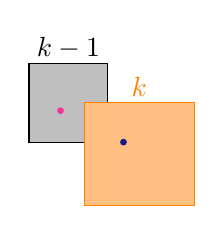
\begin{tikzpicture}
							\draw[visible on=<2->, fill=gray!50] (0, 0) rectangle (1, 1);
							\node[visible on=<2->] at (0.5, 1.2) {$k-1$};
							\filldraw[RubineRed!80, visible on=<2->] (0.4, 0.4) circle (1pt);
							\draw[orange, fill=orange!50, visible on=<3->] (0.7, 0.5) rectangle (2.1, -0.8);
							\node[visible on=<3->, orange] at (1.4, 0.7) {$k$};
							\filldraw[NavyBlue!90, visible on=<3->] (1.2, 0) circle (1pt);
						\end{tikzpicture}
					}
				\end{minipage}
			\end{frame}

		\subsection{Parameter measurements}
			\begin{frame}{Navigation}{Parameter measurements}
					\centering
					\begin{minipage}{0.6\textwidth}
						\onslide<1->{
							\begin{block}{Parameter}
								\begin{itemize}
									\item Exteroceptive parameter (magnetic, acoustic, bathymetric, ...)
									\item Give information about robot possible state
									\item Can contract the enclosing robot state
								\end{itemize}
							\end{block}
						}
						\onslide<4->{
							\begin{block}{Scope}
								\begin{itemize}
									\item Mapping known a priori
									\item Map generated by sensor or simulator
								\end{itemize}
							\end{block}
						}
					\end{minipage}
					\begin{minipage}{0.35\textwidth}
						\centering
						\resizebox*{0.8\textwidth}{!}{
							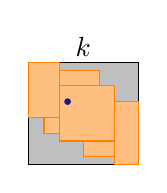
\begin{tikzpicture}
								\draw[fill=gray!50, visible on=<2->] (0.7, 0.5) rectangle (2.1, -0.8);
								\node[visible on=<2->, alt=<3->{color=orange}] at (1.4, 0.7) {$k$};
								\draw[orange, fill=orange!50, visible on=<3->] (0.7, 0.5) rectangle (1.1, -0.2);
								\draw[orange, fill=orange!50, visible on=<3->] (1.1, 0.2) rectangle (1.8, -0.5);
								\draw[orange, fill=orange!50, visible on=<3->] (0.9, -0.2) rectangle (1.1, -0.4);
								\draw[orange, fill=orange!50, visible on=<3->] (1.1, 0.4) rectangle (1.6, 0.2);
								\draw[orange, fill=orange!50, visible on=<3->] (1.8, 0) rectangle (2.1, -0.8);
								\draw[orange, fill=orange!50, visible on=<3->] (1.4, -0.5) rectangle (1.8, -0.7);

								\filldraw[NavyBlue!90, visible on=<2->] (1.2, 0) circle (1pt);
							\end{tikzpicture}
						}
					\end{minipage}
				\end{frame}

	\section{Control}

		\subsection{Prediction}
			\begin{frame}{Control}{Prediction}
				\centering
				\begin{minipage}{0.6\textwidth}
					\onslide<1->{
						\begin{block}{Prediction}
							\begin{itemize}
								\item Using estimated robot state
								\item Generate prediction at next time step using enclosing evolution and control function
							\end{itemize}
						\end{block}
					}
					\onslide<5->{
						\begin{block}{Application}
							\begin{itemize}
								\item Check the viability of the control
								\item Enclose the next estimated state
								\item Detect danger zones intersections
							\end{itemize}
						\end{block}
					}
				\end{minipage}
				\hfill
				\begin{minipage}{0.35\textwidth}
					\centering
					\resizebox*{0.8\textwidth}{!}{
						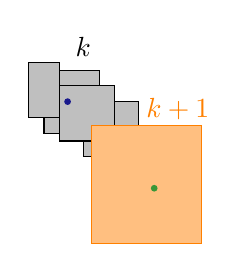
\begin{tikzpicture}
							\node[visible on=<2->] at (1.4, 0.7) {$k$};
							\draw[fill=gray!50, visible on=<2->] (0.7, 0.5) rectangle (1.1, -0.2);
							\draw[fill=gray!50, visible on=<2->] (1.1, 0.2) rectangle (1.8, -0.5);
							\draw[fill=gray!50, visible on=<2->] (0.9, -0.2) rectangle (1.1, -0.4);
							\draw[fill=gray!50, visible on=<2->] (1.1, 0.4) rectangle (1.6, 0.2);
							\draw[fill=gray!50, visible on=<2->] (1.8, 0) rectangle (2.1, -0.8);
							\draw[fill=gray!50, visible on=<2->] (1.4, -0.5) rectangle (1.8, -0.7);

							\filldraw[NavyBlue!90, visible on=<2->] (1.2, 0) circle (1pt);

							\node[orange, visible on=<3->] at (2.6, -0.1) {$k+1$};
							\draw[orange, fill=orange!50, visible on=<3>] (1.5, -0.5) rectangle (2.5, -1);
							\draw[orange, fill=orange!50, visible on=<3>] (2, -0.8) rectangle (2.7, -1.4);
							\draw[orange, fill=orange!50, visible on=<3>] (1.6, -0.9) rectangle (2.2, -1.3);
							\draw[orange, fill=orange!50, visible on=<3>] (2.1, -1.2) rectangle (2.9, -1.6);
							\draw[orange, fill=orange!50, visible on=<3>] (2.3, -1.4) rectangle (2.6, -1.8);
							\draw[orange, fill=orange!50, visible on=<3>] (1.8, -0.3) rectangle (2.4, -0.7);
							
							\draw[orange, fill=orange!50, visible on=<4->] (1.5, -0.3) rectangle (2.9,-1.8);

							\filldraw[ForestGreen!90, visible on=<3->] (2.3, -1.1) circle (1pt);
						\end{tikzpicture}
					}
				\end{minipage}
			\end{frame}

		\subsection{Control}
			\begin{frame}{Control}{Control}
				\centering
				\begin{minipage}{0.6\textwidth}
					\onslide<1->{
						\begin{block}{Control}
							\begin{itemize}
								\item Generate control using enclosing control function on estimated state
								\item Take the barycenter of control as inputs
							\end{itemize}
						\end{block}
					}
					\onslide<6->{
						\begin{block}{Results}
							\begin{itemize}
								\item Control roughly the robot
								\item Gives correct results
							\end{itemize}
						\end{block}
					}
				\end{minipage}
				\hfill
				\begin{minipage}{0.35\textwidth}
					\centering
					\resizebox*{0.8\textwidth}{!}{
						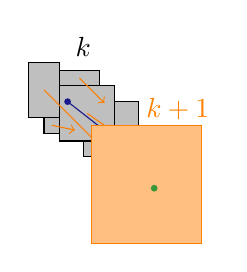
\begin{tikzpicture}
							\node[visible on=<2->] at (1.4, 0.7) {$k$};
							\draw[fill=gray!50, visible on=<2->] (0.7, 0.5) rectangle (1.1, -0.2);
							\draw[fill=gray!50, visible on=<2->] (1.1, 0.2) rectangle (1.8, -0.5);
							\draw[fill=gray!50, visible on=<2->] (0.9, -0.2) rectangle (1.1, -0.4);
							\draw[fill=gray!50, visible on=<2->] (1.1, 0.4) rectangle (1.6, 0.2);
							\draw[fill=gray!50, visible on=<2->] (1.8, 0) rectangle (2.1, -0.8);
							\draw[fill=gray!50, visible on=<2->] (1.4, -0.5) rectangle (1.8, -0.7);

							\filldraw[NavyBlue!90, visible on=<2->] (1.2, 0) circle (1pt);
							
							\draw[-to, >=latex, orange, visible on=<3>] (0.9, 0.15) -- +(-45:1);
							\draw[-to, >=latex, orange, visible on=<3>] (1.45, -0.15) -- +(-35:0.6);
							\draw[-to, >=latex, orange, visible on=<3>] (1, -0.3) -- +(-12:0.3);
							\draw[-to, >=latex, orange, visible on=<3>] (1.35, 0.3) -- +(-45:0.45);
							\draw[-to, >=latex, orange, visible on=<3>] (1.95, -0.4) -- +(-25:0.4);
							\draw[-to, >=latex, orange, visible on=<3>] (1.6, -0.6) -- +(-15:0.6);

							\draw[-to, >=latex, NavyBlue!90, visible on=<4>] (1.2, 0) -- +(-38:0.85);
							
							\node[orange, visible on=<5->] at (2.6, -0.1) {$k+1$};
							\draw[orange, fill=orange!50, visible on=<5->] (1.5, -0.3) rectangle (2.9,-1.8);
							\filldraw[ForestGreen!90, visible on=<5->] (2.3, -1.1) circle (1pt);
						\end{tikzpicture}
					}
				\end{minipage}
			\end{frame}

	\section{Example}

		\subsection{Boat}
			\begin{frame}{Example}{Formalism}
				\centering
				\begin{minipage}{0.6\textwidth}
					\begin{block}{Scope of the example}
						\begin{itemize}
							\item Boat simulated with Dubins state equation
							\item Using simulated bathymetric map as measured field
							\item Control the boat to follow a Lissajous curve
						\end{itemize}
					\end{block}
					\begin{block}{Assumptions}
						\begin{itemize}
							\item State estimation and control only using interval analysis
							\item Inertial drift set to $0.1\ m$ per seconds
							\item Bathymetric measurements uncertainty set to $0.1\ m$
						\end{itemize}
					\end{block}
				\end{minipage}
			\end{frame}

			\begin{frame}{Example}{Simulation}
				\centering
				\begin{figure}
					\movie{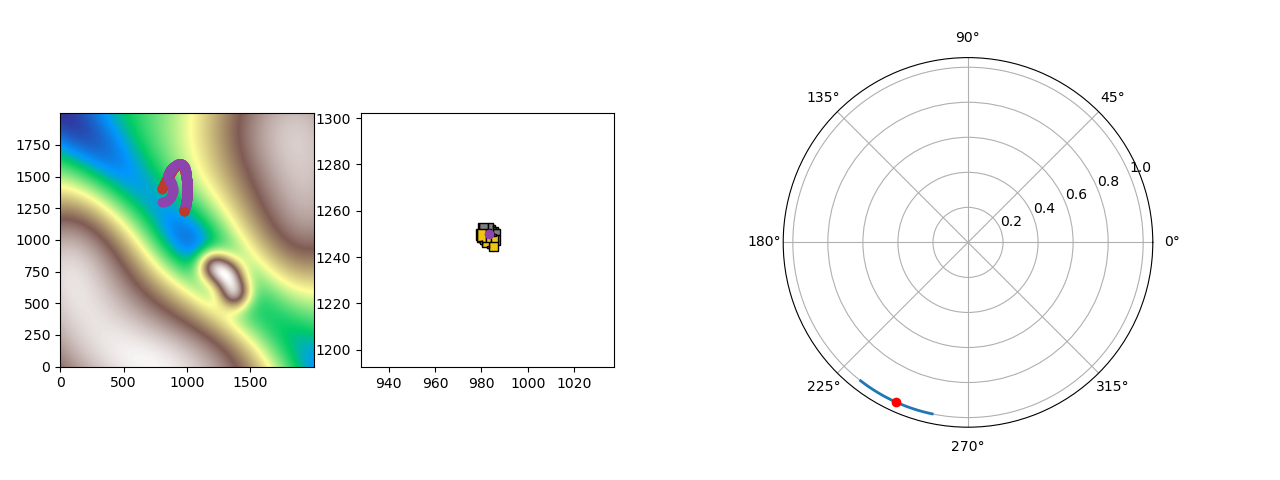
\includegraphics[width=\textwidth]{images/cover.png}}{navigation.mp4}
				\end{figure}
			\end{frame}

			\begin{frame}{Example}{Conclusion}
				\centering
				\begin{minipage}[c]{0.6\textwidth}
					\begin{block}{Innovation}
						\begin{itemize}
							\item Complete control loop using set methods
							\item Easy sensor data fusion
							\item Safe and resilient control
						\end{itemize}
					\end{block}
					\begin{block}{Conclusion}
						\begin{itemize}
							\item Works better in highly nonlinear fields
							\item Possibility to refine next state estimation by enclosing it in a sub-paving
							\item Still a simulation will be tried in guaranteed robot control experiments.
						\end{itemize}
					\end{block}
				\end{minipage}
				\hfill
				\begin{minipage}[c]{0.3\textwidth}
					\begin{figure}
						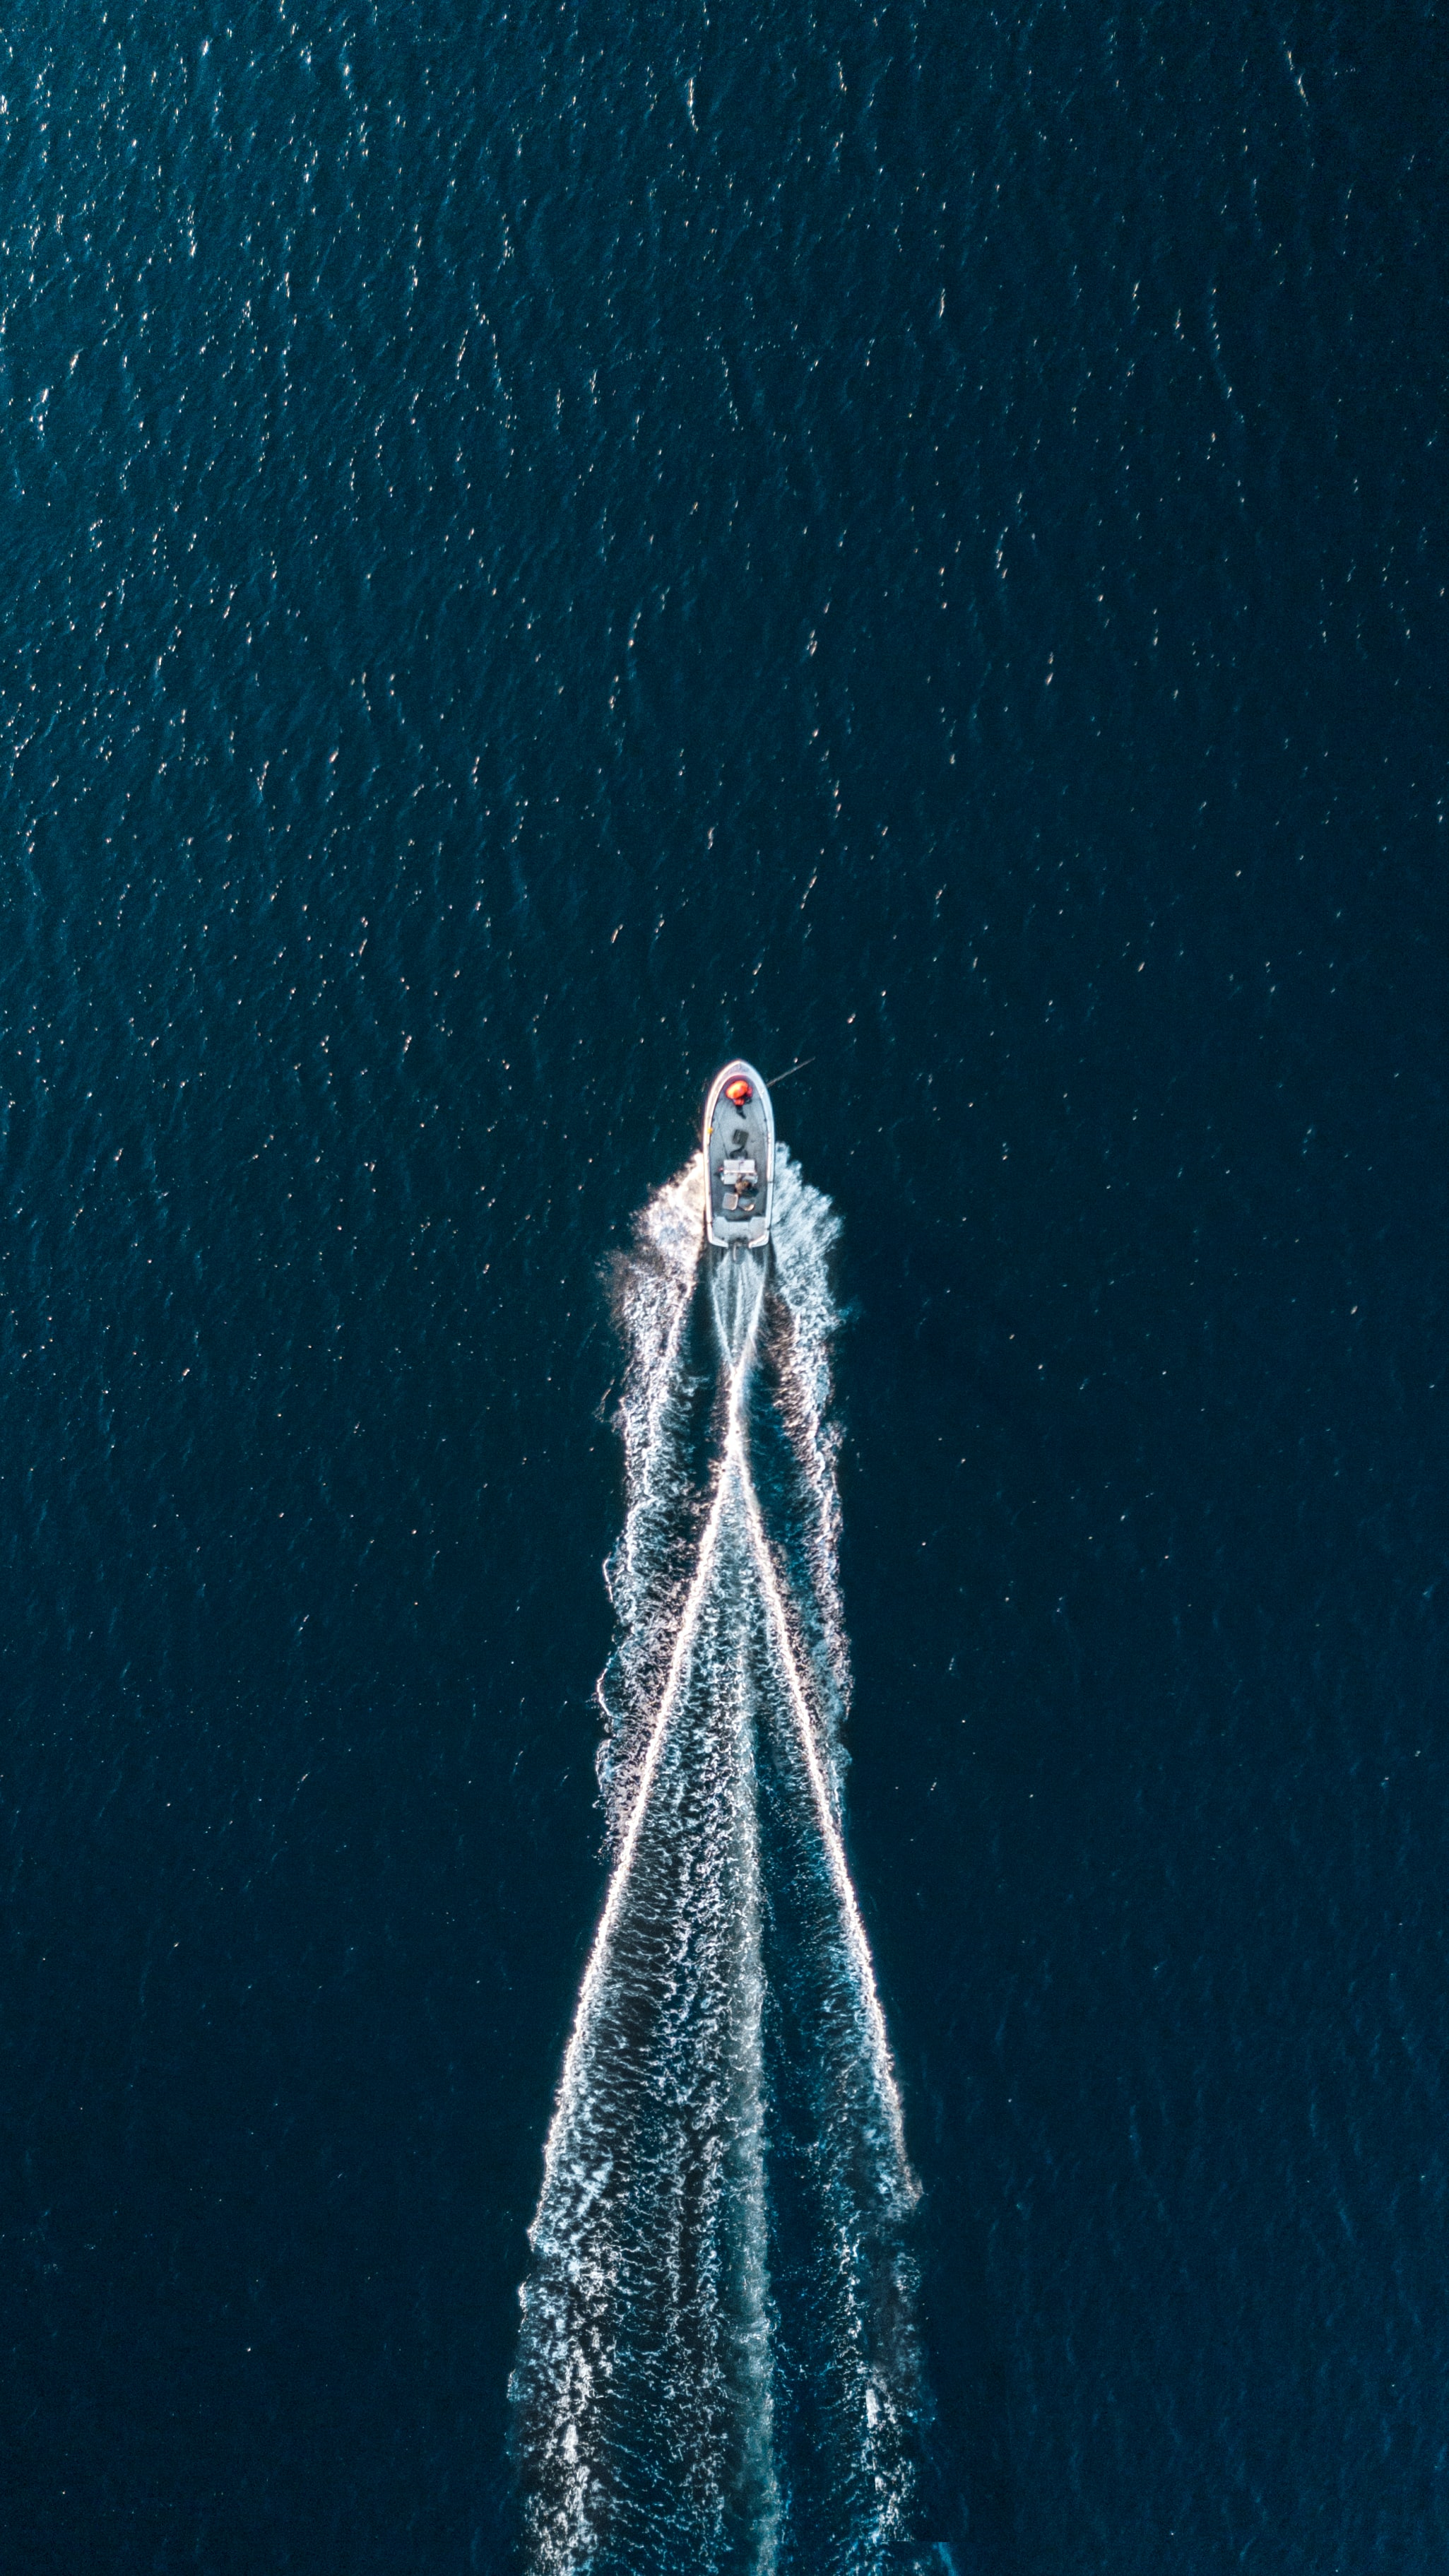
\includegraphics[width=\textwidth]{images/boat_end.jpg}
						\caption{Sailing boat}
					\end{figure}
				\end{minipage}
			\end{frame}
\end{document}